\section{Définitions}
\begin{defi}%Fonctions récusives]
Une fonction récursive est une fonction qui s'appelle elle-même.

On appelle récursion l'appel de la fonction à elle-même.
\end{defi}

La programmation est un paradigme de programmation au même titre que la programmation itérative. Un programme écrit de manière récursive peut être traduit de manière itérative, même si dans certain cas, cela peut s'avérer délicat.


\begin{methode}
\begin{itemize}
\item Une fonction récursive doit posséder une condition d'arrêt (ou cas de base).
\item Une fonction récursive doit s'appeler elle-même (récursion).
\item L'argument de l'étape de récursion doit évoluer de manière à se ramener à la condition d'arrêt.
\end{itemize}
\end{methode}
 
 



\section{Suites définies par récurrence}

Les suite définies par récurrence pour les quelles $u_{n}=f\left(u_{n-1},u_{n-2},...\right)$ sont des cas d'application directs des fonctions récursives. 

Par exemple, soit la suite $u_n$ définie par récurrence pour tout $n\in\mathbb{N}^*$ par 
$
\left\{
\begin{array}{ll} 
u_1 = 1 \\
u_{n+1} = \dfrac{u_n + 6}{u_n + 2} \\
\end{array}
\right.
$. Il est possible de calculer le n\ieme terme par un algorithme itératif ou un algorithme récursif. 

\noindent\begin{minipage}[c]{.45\linewidth}
\begin{lstlisting}
def un_it (n : int) -> float :
    if n == 1 :
        return 1
    else : 
        u = 1
        for i in range(2,n+1):
            u = (u+6)/(u+2)
        return u
\end{lstlisting}
\end{minipage} \hfill
\begin{minipage}[c]{.45\linewidth}
\begin{lstlisting}
def un_rec (n : int) -> float :
    if n == 1 :
        return 1
    else : 
        return (un_rec(n-1)+6)/(un_rec(n-1)+2)
\end{lstlisting}
\end{minipage} 

La figure suivante montre que dans le cas de l'algorithme récursif proposé plusieurs termes sont calculés à plusieurs reprises ce qui constitue une perte de temps et d'espace mémoire. 

\begin{center}
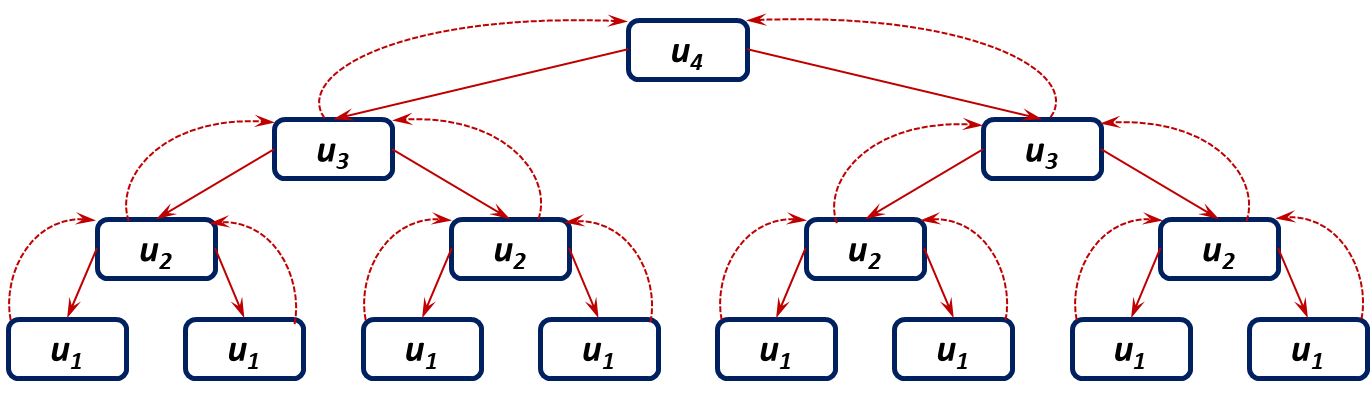
\includegraphics[width=.8\linewidth]{fig_01}
\end{center}

Une autre formulation de l'algorithme récursif permet très simplement de diminuer le nombre de termes calculés. 



\noindent\begin{minipage}[c]{.45\linewidth}
\begin{lstlisting}
def un_rec (n : int) -> float :
    if n == 1 :
        return 1
    else : 
        v = un_rec(n-1)
        return (v+6)/(v+2)
\end{lstlisting}
\end{minipage} \hfill
\begin{minipage}[c]{.45\linewidth}
\begin{center}
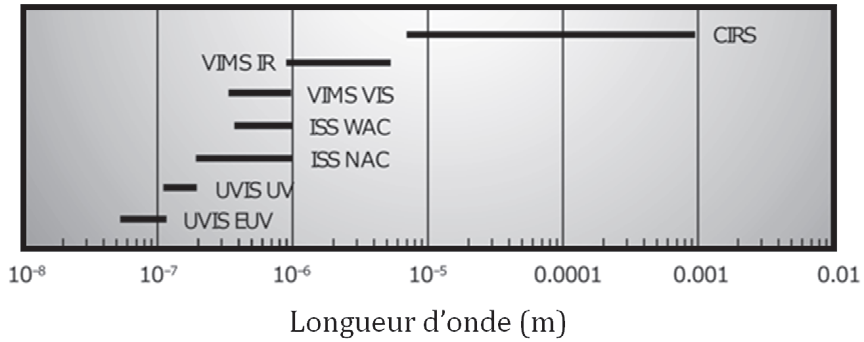
\includegraphics[width=.8\linewidth]{fig_02}
\end{center}\end{minipage}

\section{Algorithmes dichotomiques -- Divisier pour régner}

Les algorithmes dichotomiques se prètent aussi à des formulations récursives. Prenons comme exemple la recherche d'un élément dans une liste triée. L'algorithme de gauche propose une version itérative. L'algorithme de droite une version récursive. 

\noindent\begin{minipage}[c]{.49\linewidth}
\begin{lstlisting}
def appartient_dicho(e : int , t : list) -> bool:
    """Renvoie un booléen indiquant si e est 
    dans t. Préconditions : t est un tableau 
    de nombres trié par ordre croissant e est 
    un nombre"""
    # Limite gauche de la tranche où l'on recherche e
    g = 0 
    # Limite droite de la tranche où l'on recherche e
    d = len(t)-1 
    # La tranche où l'on cherche e n'est pas vide
    while g <= d: 
        # Milieu de la tranche où l'on recherche e
        m = (g+d)//2 
        pivot = t[m]
        if e == pivot: # On a trouvé e
            return True
        elif e < pivot:
            # On recherche e dans la partie gauche de la tranche
            d = m-1 
        else:
            # On recherche e dans la partie droite de la tranche
            g = m+1 
    return False
\end{lstlisting}
\end{minipage} \hfill
\begin{minipage}[c]{.49\linewidth}
\begin{lstlisting}
def appartient_dicho_rec(e : int , t : list) -> bool:
    """Renvoie un booléen indiquant si e est dans t. Préconditions : t est un tableau de nombres trié par ordre croissant e est un nombre"""
    # Limite gauche de la tranche où l'on recherche e
    g = 0 
    # Limite droite de la tranche où l'on recherche e
    d = len(t)-1 
    # La tranche où l'on cherche e n'est pas vide
    while g <= d:
        # Milieu de la tranche où l'on recherche e 
        m = (g+d)//2 
        pivot = t[m]
        if e == pivot: # On a trouvé e
            return True
        elif e < pivot:
            # On recherche e dans la partie gauche de la tranche
            d = m-1 
            appartient_dicho_rec(e,t[g:d])
        else :
            # On recherche e dans la partie droite de la tranche
            g = m+1
            appartient_dicho_rec(e,t[g:d])
    return False
\end{lstlisting}
\end{minipage}

\section{Tracer de figures définies par récursivite}
Un grand nombre de figures peuvent être tracés en utilisant des algorithmes récursifs (flocon de Koch, courbe de Peano, courbe du dragon \textit{etc.}).


\begin{lstlisting}
import matplotlib.pyplot as plt
import numpy as np
def cercle(x,y,r):
    theta = np.linspace(0, 2*np.pi, 100)  #des points régulièrement espacés dans l'intervalle [0,2pi]
    X = [x+r*np.cos(t) for t in theta]      #abscisses de points du cercle C((x,y),r)
    Y = [y+r*np.sin(t) for t in theta]       #ordonnées de points du cercle C((x,y),r)
    plt.plot(X,Y,"b")     #tracé sans affichage
\end{lstlisting}

\noindent\begin{minipage}[c]{.49\linewidth}
\begin{lstlisting}
def bubble(n, x, y, r, d):
    cercle(x, y, r)
    if n > 1:
        if d != 's':
            bubble(n-1,x,y+3*r/2,r/2,"n")
        if d != 'w':
            bubble(n-1,x+3*r/2,y,r/2,"e")
        if d != 'n':
            bubble(n-1,x,y-3*r/2,r/2,"s")
        if d != 'e':
            bubble(n-1,x-3*r/2,y,r/2,"w")
bubble(4,0,0,8,"")
plt.axis("equal")
plt.show()
\end{lstlisting}
\end{minipage} \hfill
\begin{minipage}[c]{.49\linewidth}
\begin{center}
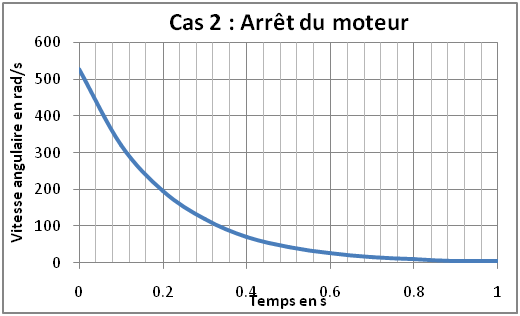
\includegraphics[width=\linewidth]{fig_03}
\end{center}
\end{minipage}
%\subsection{Exponentiation rapide}
%L'exponentiation rapide est un algorithme permettant de calculer $x^n$ en utilisant l'algorithme récursif suivant : 
%$
%\text{puissance}(x,n) =
%\left\{
%\begin{array}{ll}
%x & \text{si }n=1 \\
%\text{puissance}(x^2,n/2) & \text{si } $n$ \text{ est pair} \\
%x\times \text{puissance}(x^2,(n-1)/2) & \text{si } $n$ \text{ est impar pair} \\
%\end{array}
%\right.
%.$
%
%\noindent\begin{minipage}[c]{.45\linewidth}
%\begin{lstlisting}
%def expo_it(x : float, n : int) -> float :
%    res=1
%    while n!=0:
%        if n%2==1:
%            res = res*x
%        x*=x
%        n//=2
%    return res
%\end{lstlisting}
%\end{minipage} \hfill
%\begin{minipage}[c]{.45\linewidth}
%\begin{lstlisting}
%def expo_rec(x : float, n : int) -> float :
%    if n==0:
%        return 1
%    elif n%2==0:
%        return expo_rec(x*x,n//2)
%    else:
%        return x*expo_rec(x*x,n//2)
%\end{lstlisting}
%\end{minipage} 
%



\section{Activité préparatoire}
\textbf{Pour réaliser l'activité associée à ce cours, suivre le lien suivant : }
\begin{itemize} 
\item Sujet : \url{https://bit.ly/3zkiJgb}
\item Corrige : \url{https://bit.ly/3zl7QKJ}
\end{itemize}

\newpage
\section{QCM}

\question{Que retourne la commande suivante \texttt{mystere(4)} ?}
\begin{lstlisting}
def mystere(n):
    if n>0 :
        return mystere(n-2)
    else :
        return n==0
\end{lstlisting}

\begin{enumerate}
\item 0.
\item False.
\item True. % +
\item L'exécution génère une erreur.
\end{enumerate}

\question{Laquelle de ces fonctions retourne True lorsqu'on exécute \texttt{f(5)} ?}
\begin{lstlisting}
def f1(n):
    if n==0 :
        return True
    else :
        return f(n-2)
        
def f2(n):
    if n<=0 :
        return True
    else :
        f(n-2)
        
def f3(n):
    if n<=0 :
        return True
    return f(n-2)

def f4(n):
    if n==0 :
        return True
    f(n-2)
\end{lstlisting}


\begin{enumerate}
\item \texttt{f1}.
\item \texttt{f2}.
\item \texttt{f3}. %+
\item \texttt{f4}.
\end{enumerate}

\question{ Quel affichage obtient-on en exécutant \texttt{affiche(3)} ?}
\begin{lstlisting}
def affiche(n):
    print(n)
    if n>=0:
        affiche(n-1)
\end{lstlisting}

\begin{enumerate}
\item 3, 2, 1, 0 (avec des retours à la ligne entre chaque valeurs).
\item 0, 1, 2, 3 (avec des retours à la ligne entre chaque valeurs).
\item 3, 2, 1, 0, -1 (avec des retours à la ligne entre chaque valeurs). %+
\item 3.
\end{enumerate}

\question{Une seule des fonctions définies ci-dessous retourne \texttt{'ccccc'} à l'appel de \texttt{replique(5,'c')}. Déterminer laquelle.}
\begin{lstlisting}
def replique(a,b): # Fonction 1
    if a==1:
        return b
    else :
        return replique( a-1 , b+b)

def replique(a,b): # Fonction 2
    if a==1:
        return b
    elif a%2 == 0:
        return replique( a-2 , b+b)
    else :
        return b + replique( a-2 , b+b)

def replique(a,b): # Fonction 3
    if a==1:
        return b
    elif a%2 == 0:
        return replique( a//2 , b+b)
    else :
        return b + replique( a//2 , b+b)

def replique(a,b): # Fonction 4
    if a==1:
        return b
    else :
        replique( a-1 , b+b)
\end{lstlisting}

\begin{enumerate}
\item Fonction 1.
\item Fonction 2.
\item Fonction 3.
\item Fonction 4.
\end{enumerate}

\question{Que retourne l'instruction \texttt{copy(3,'A')} ?}
\begin{lstlisting}
def copy(n,s):
    if n==0:
        return s
    return copy(n-1, s+s)
\end{lstlisting}

\begin{enumerate}
\item \texttt{'AAA'}.
\item \texttt{'AAAAAA'}.
\item \texttt{'AAAAAAAA'}.
\item \texttt{'3A'}.
\end{enumerate}

\question{Que retourne l'instruction : \texttt{mystere(3,'\$')} ?}
\begin{lstlisting}
def mystere(n,s):
    if n==0:
        return s
    return s + mystere(n-1, s)
\end{lstlisting}

\begin{enumerate}
\item \texttt{'\$\$\$'}.
\item \texttt{'\$2\$'}.
\item \texttt{'\$\$\$\$'}. %+
\item L'exécution déclenche une erreur.
\end{enumerate}

\question{Que retourne la commande \texttt{f(3,4)} ?}
\begin{lstlisting}
def f(a,b):
    if a == 0 :
        return b
    return f(a-1, b+1)
\end{lstlisting}

\begin{enumerate}
\item 4.
\item 5.
\item 6.
\item 7. %+
\end{enumerate}

\question{Que retourne la commande \texttt{mystere(3)} ?}
\begin{lstlisting}
def mystere(n):
    if n>0 :
        return mystere(n-2)
    else :
        return n==0
\end{lstlisting}

\begin{enumerate}
\item True.
\item False. %+
\item RecursionError.
\item 0.
\end{enumerate}

\question{On propose de créer une fonction récursive permettant de calculer  $x^n$. Compléter la fonction proposée.}
\begin{lstlisting}
def puissance(x,n):
    if n > 0 : 
        return .......
    return 1
\end{lstlisting}

\begin{enumerate}
\item \texttt{puissance(x,n-1)}.
\item \texttt{x*puissance(x,n-1)}. %+
\item Quoi que l'on écrive, cette fonction ne donnera pas le résultat attendu.
\item \texttt{x**(n-1)*puissance(x,n-1)}.
\end{enumerate}

\question{Que renvoi ce programme en console ?}
\begin{lstlisting}
def ed(L,M=[]):
    if len(L) == 0 : return M
    a=L.pop()
    if a not in M : M.append(a)
    return ed(L,M)
L=[2, 3, 2, 6, 8, 9, 9, 10, 9, 3, 6, 7, 8, 8, 9]
print(ed(L))
\end{lstlisting}

\begin{enumerate}
\item \texttt{None}.
\item \texttt{[9, 8, 7, 6, 3, 10, 2]}. %+
\item \texttt{[9, 8, 8, 7, 6, 3, 9, 10, 9, 9, 8, 6, 2, 3, 2]}.
\item \texttt{[2, 10, 3, 6, 7, 8, 9]}.
\end{enumerate}

\question{Que retourne le programme suivant ?}
\begin{lstlisting}
def A(x):
    if x <= 1 : return x
    return B(x+1)

def B(x) :
    return A(x-2)+4

print(A(4))
\end{lstlisting}

\begin{enumerate}
\item 13. %+
\item 1.
\item 12.
\item Une erreur de type : "RecursionError: maximum recursion depth exceeded in comparison".
\end{enumerate}
